\documentclass[12pt]{article}


\usepackage{fullpage}
\usepackage{amsmath}
\usepackage{amssymb}
\usepackage{color}
\date{}

\newcommand{\mys}[2]{\displaystyle\sum_{#1}^{#2}}

\usepackage{tikz}

\newif\ifans
\anstrue


\begin{document}

\begin{center}
  \textbf{COMS 3110: Homework 1}\\
  \textbf{Due: September $20^{th}$, 11:59pm}\\
  \textbf{Total Points: 40}
\end{center}


\paragraph{Late submission policy.\ }
An assignment that is submitted one day late will get a penalty of $10\%$. An assignment that is submitted two days late will get a penalty of $20\%$. Assignments submitted after two days will not be graded and will get no points. For example, if an assignment is due on Friday by midnight, a submission on Saturday will be penalized by $10\%$, and a submission on Sunday will be penalized by $20\%$. A submission on Monday will get no points. 

\paragraph{Submission format.\ }
Homework solutions will have to be typed. You can use word, LaTeX, or any other type-setting tool to type your solution. Your submission file should be in pdf format. Do \textbf{NOT} submit a photocopy of handwritten homework except for diagrams that can be hand-drawn and scanned. We reserve the right \textbf{NOT} to grade homework that does not follow the formatting requirements.
Name your submission
file: \texttt{<Your-net-id>-3110-hw1.pdf}. For instance, if your netid
is \texttt{asterix}, then your submission file will be named
\texttt{asterix-3110-hw1.pdf}.
Each student must hand in their own assignment. If you discussed the homework or solutions with others, a list of collaborators must be included with each submission. Each of the collaborators has to write the solutions in their own words (copies are not allowed).

\paragraph{General Requirements}
\begin{itemize}
    \item When proofs are required, do your best to make them both clear and rigorous. Even when proofs are not required, you should justify your answers and explain your work.
    \item When asked to present a construction, you should show the correctness of the construction.
\end{itemize}

\paragraph{Some Useful (in)equalities}
\begin{itemize}
    \item $\sum_{i=1}^n i= \frac{n(n+1)}{2}$
    \item $\sum_{i=1}^ni^2 = \frac{n(n+1)(2n+1)}{6}$
    \item $2^{\log_2n}=n$, $a^{\log_bn}=n^{\log_ba}$, $n^{n/2}\leq n! \leq n^n$, $\log x^a = a\log x$
    \item $\log (a\times b) = \log a + \log b$, $\log(a/b) = \log a - \log b$
    \item $a + ar + ar^2 + ... + ar^{n-1} = \frac{a(r^n-1)}{r-1}$
    \item $1 + \frac{1}{2} + \frac{1}{2^2} + ... + \frac{1}{2^n} = 2(1-\frac{1}{2^{n+1}})$
    \item $1 + 2 + 4 + ... + 2^n = 2^{n+1}-1$
\end{itemize}


% \hrule

% \newpage

\begin{enumerate}
\item
  \textbf{(5 pts)} Prove $\left[\frac{n(n+1)}{2}\right]^2-\frac{n^2(n^2+1)}{4}+98\in O(n^3)$.

\item
  \textbf{(5 pts)} Prove or disprove $2^{2^n} \in O(2^{2n})$. 

\item \label{prob:courses}
  \textbf{(5 pts)} Prove that any function that is in $O(\log_2n)$ is also in $O(\log_3n)$.

\item \textbf{(5 pts)} Prove that if $f_1(n) \in O(g_1(n))$ and $f_2(n) \in O(g_2(n))$, then
    \boldmath
    \begin{equation*}
        f_1(n) + f_2(n) \in O(g_1(n) + g_2(n))
    \end{equation*}
    \unboldmath

\item \textbf{(10 pts)} Derive the runtime of the following loop structure as a function of $n$ and determine its Big-O upper bound. You must show the derivation of the end result. Simply stating the final answer without any derivation steps will result in zero points. Assume atomic operations take unit time.
\begin{center}
    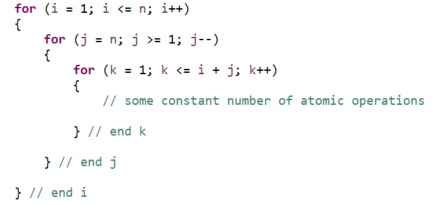
\includegraphics[scale=1.4]{hw1_pic1.png}
\end{center}

\item \textbf{(10 pts)}
  Derive the runtime of the following loop structure as a function of $n$ and determine its Big-O upper bound. You must show the derivation of the end result. Simply stating the final answer without any derivation steps will result in zero points. Assume atomic operations take unit time.
  \begin{center}
    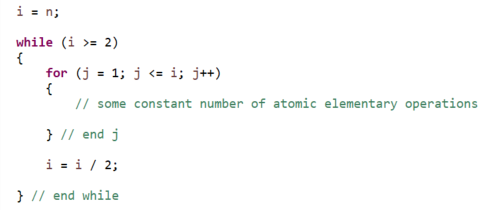
\includegraphics[scale=1.3]{hw1_pic2.png}
  \end{center}

\end{enumerate}


\end{document}




%%% Local Variables:
%%% mode: latex
%%% TeX-master: t
%%% End:
